\part{IHM}
\setcounter{section}{0}

\section{Enchainement des fenêtres - EDF}

\begin{figure}[H]
\noindent\makebox[\textwidth]{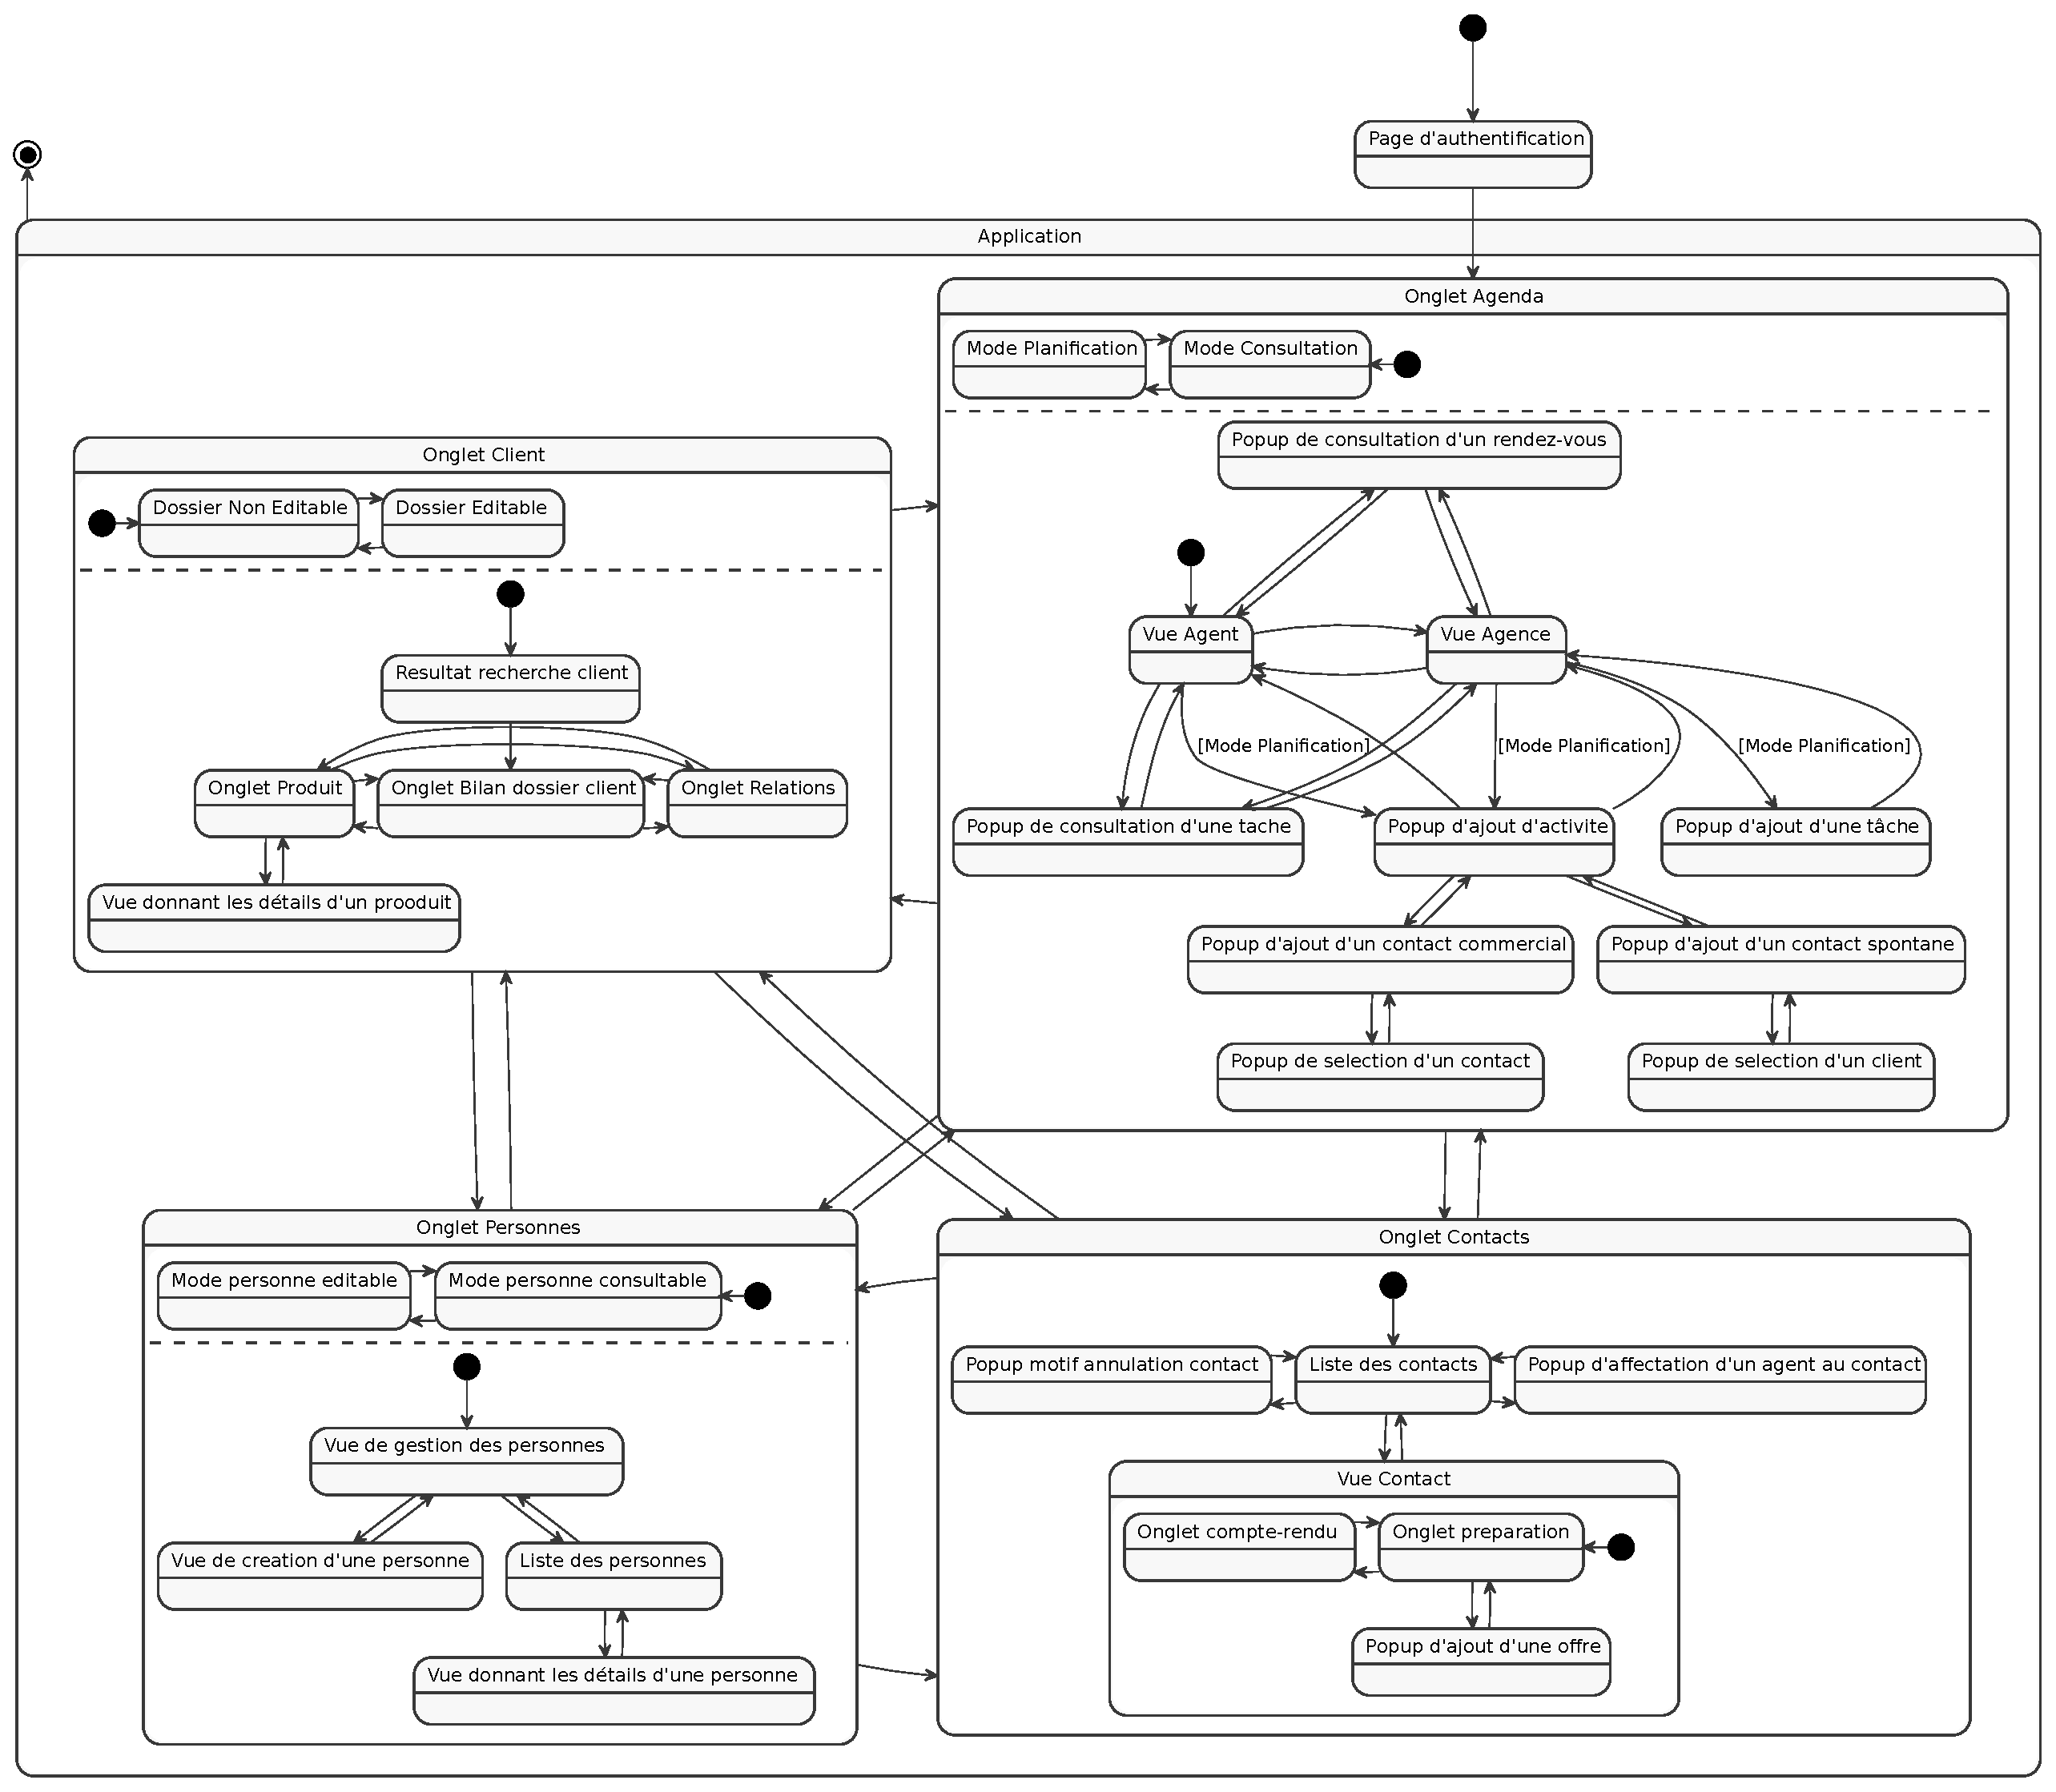
\includegraphics[width=18cm]{figures/eps/EdF}}
\caption{Diagramme d'enchainement des fenêtres}
\end{figure}

\section{Présentation des différentes vues}
Les vues de l'IHM sont présentées dans les pages suivantes.

\begin{shaded}
\textbf{Note: } Les tableaux récapitulant les SMA des différentes vues sont présentés par IHM. Si des services sont redondants, ils ont le même numéro et ne sont pas répétés dans le tableau. \\

Les cas d'utilisation des IHM sont indiqués en haut à gauche de chaque vue. La description des CU n'a pas été reportée en dessous des fenêtres. Dans le cas de manipulation qui ne sont pas immédiatement visibles, ou qui auraient engendrées une trop grosse redondance des vues, nous avons placé des commentaires sur les bords.
\end{shaded}

\includepdf[scale=0.8,angle=90,pages={2-9},pagecommand=\subsection*{IHM client}]{figures/IHM.pdf}


\begin{table}[H]
\centering
\caption{SMA - IHM Client}
\begin{tabular}{p{0.1\textwidth}p{0.4\textwidth}p{0.4\textwidth}}
\hline
Num & \multicolumn{1}{c}{Nom Contrôle} & \multicolumn{1}{c}{SMA} \\ \hline
\rowcolor[gray]{0.9}
\multicolumn{3}{l}{CU10 - Recherche des clients}  \\
1.1 & Bouton Rechercher & PAS DE SMA \\
\rowcolor[gray]{0.9}
\multicolumn{3}{l}{CU10 - Résultats recherche clients} \\ 
1.2 & Bouton Rechercher  & PAS DE SMA       \\             
1.3 & Bouton Voir le client & ObtenirClientEtAgence \newline ConsulterBilanClient \\
\rowcolor[gray]{0.9}
\multicolumn{3}{l}{CU10 - Bilan - Dossier Client}  \\
1.4 & bouton oeil  & ConsulterDetailPersonne \\
1.5 & bouton crayon  & ConsulterDetailPersonne \\
1.6 & bouton poubelle  & SupprimerPersonne \\
1.7 & onglet Produits  & ObtenirProduits \\
1.8 & onglet Relations  & ConsulterRelationsBanqueClient \\
\rowcolor[gray]{0.9}
\multicolumn{3}{l}{CU10 - Bilan - Dossier Client- Mode modification} \\ 
1.9 & Bouton Ajouter une personne  &  AjouterPersonne ou \newline CreerEtAjouterPersonne  \\             
1.10 & Bouton Enlever du client & SupprimerPersonne \\
1.11 & Bouton Valider & MAJEnteteDossier \\
\rowcolor[gray]{0.9}
\multicolumn{3}{l}{CU10 - Produits - Dossier client}  \\
1.12 & onglet Bilan & ConsulterBilanClient \\
1.13 & Bouton oeil & ConsulterDetailProduit \\
1.14 & Bouton Modifier (puis valider) & MAJComptesConcurrence \\
\rowcolor[gray]{0.9}
\multicolumn{3}{l}{CU10 - Détail produit - Dossier client} \\ 
\rowcolor[gray]{0.9}
\multicolumn{3}{l}{CU10 - Relations - Dossier client} \\ \hline
\end{tabular}
\end{table}


\includepdf[scale=0.8,angle=90,pages={10-14},pagecommand=\subsection*{IHM Personnes}]{figures/IHM.pdf}

\begin{table}[H]
\centering
\caption{SMA - IHM Personnes}
\begin{tabular}{ll}
\hline
\multicolumn{1}{c}{Num Contrôle} & \multicolumn{1}{c}{SMA} \\ \hline
\multicolumn{2}{c}{CU2 - Affectation contact}              \\
                                 &                         \\
                                 &                         \\ \hline
\end{tabular}
\end{table}


\includepdf[scale=0.8,angle=90,pages={15-25},pagecommand=\subsection*{IHM Agenda}]{figures/IHM.pdf}

\begin{table}[H]
\centering
\caption{SMA - IHM Agenda}
\begin{tabular}{p{0.1\textwidth}p{0.4\textwidth}p{0.4\textwidth}}
\hline
Num & \multicolumn{1}{c}{Nom Contrôle} & \multicolumn{1}{c}{SMA} \\ \hline
\rowcolor[gray]{0.9}
\multicolumn{3}{l}{CU7 - Agenda - Agence}  \\
3.1 & Bouton Vue Agent & ObtenirAgendaAgent \\
\rowcolor[gray]{0.9}
\multicolumn{3}{l}{CU7 - Agenda - Agent}  \\
3.2 & Bouton Vue Agence & ObtenirAgendaAgence \\
3.3 & ComboBox Agent & ObtenirAgendaAgent \\
\rowcolor[gray]{0.9}
\multicolumn{3}{l}{CU7 - Agenda - Ajout plage horaire chef d'agence}  \\
3.4 & Ajouter une activité & ObtenirAgendaAgence \\
3.3 & ComboBox Agent & ObtenirAgendaAgent \\
\rowcolor[gray]{0.9}
\multicolumn{3}{l}{CU7 - Agenda - Ajout plage horaire agent}  \\
\rowcolor[gray]{0.9}
\multicolumn{3}{l}{CU7 - Agenda - Ajout contact}  \\
\rowcolor[gray]{0.9}
\multicolumn{3}{l}{CU7 - Agenda - Ajout contact spontané}  \\
\rowcolor[gray]{0.9}
\multicolumn{3}{l}{CU7 - Agenda - Ajout contact - recherche contact}  \\
\rowcolor[gray]{0.9}
\multicolumn{3}{l}{CU7 - Agenda - Ajout contact spontané - recherche client}  \\
\rowcolor[gray]{0.9}
\multicolumn{3}{l}{CU7 - Agenda - Ajout tâche}  \\
\rowcolor[gray]{0.9}
\multicolumn{3}{l}{CU7 - Agenda - clic tâche}  \\
\rowcolor[gray]{0.9}
\multicolumn{3}{l}{CU7 - Agenda - clic rendez-vous}  \\
\end{tabular}
\end{table}

\includepdf[scale=0.8,angle=90,pages={26-34},pagecommand=\subsection*{IHM Contact}]{figures/IHM.pdf}

\begin{table}[H]
\centering
\caption{SMA - IHM Contact}
\begin{tabular}{ll}
\hline
\multicolumn{1}{c}{Num Contrôle} & \multicolumn{1}{c}{SMA} \\ \hline
\multicolumn{2}{c}{CU2 - Affectation contact}              \\
                                 &                         \\
                                 &                         \\ \hline
\end{tabular}
\end{table}